% PCCSL 507 Machine Learning Lab - Experiment 6 (NumPy only)
\documentclass[11pt,twoside]{article}

\usepackage[paper=letterpaper,top=0.7in,bottom=0.63in,left=0.75in,right=0.75in,headheight=24pt,headsep=0.14in,footskip=0.38in]{geometry}

\usepackage[T1]{fontenc}
\usepackage{mathptmx} % Times clone
\usepackage{xcolor}
\definecolor{primary}{HTML}{1F3864}
\usepackage{fancyhdr}
\usepackage{array}
\usepackage{colortbl}
\usepackage{parskip}
\setlength{\parindent}{0pt}
\setlength{\parskip}{4pt}
\setlength{\abovedisplayskip}{4pt}
\setlength{\belowdisplayskip}{4pt}
\setlength{\abovedisplayshortskip}{2pt}
\setlength{\belowdisplayshortskip}{2pt}
\usepackage{graphicx}
\usepackage{amsmath}
\usepackage{listings}
\lstset{basicstyle=\footnotesize\ttfamily, breaklines=true, frame=single, showstringspaces=false}

\pagestyle{fancy}
\fancyhf{}
\fancyhead[C]{\textcolor{primary}{\textbf{\small PCCSL 507 Machine Learning Laboratory Record}}}
\renewcommand{\headrulewidth}{0.75pt}
\renewcommand{\headrule}{\hbox to\headwidth{\color{primary}\leaders\hrule height \headrulewidth\hfill}}
\fancyfoot[C]{\footnotesize DEPARTMENT OF CSE \hfill CAPE COLLEGE OF ENGINEERING ALAPPUZHA \hfill Page No. \thepage}
\renewcommand{\footrulewidth}{0pt}

\newcommand{\expheading}[1]{{\fontsize{14}{17}\selectfont\textbf{#1}\par}}
\newcommand{\fullrule}{\noindent\rule{\textwidth}{0.6pt}\par}

\begin{document}
\sloppy

% Sheet-local tightening so it fits one right-side page
{\setlength{\parskip}{1pt}\setlength{\abovedisplayskip}{2pt}\setlength{\belowdisplayskip}{2pt}
\begin{center}
\expheading{EXPERIMENT NO. 6}
\end{center}
\vspace{2pt}

\noindent\textbf{Date:} \underline{\hspace{2.6cm}} \hfill \textbf{Page No.:} \underline{\hspace{2.6cm}}\par
\vspace{6pt}

\expheading{TITLE}
\vspace{4pt}
\noindent Multiple Linear Regression -- House Price from Area and Age\par
\vspace{4pt}

\expheading{OBJECTIVE}
\vspace{2pt}
\fullrule
\vspace{4pt}
\noindent To predict house selling price from area and age using multiple linear regression with the normal equation, and evaluate it with MSE and R-squared with a 3D plot. \par
\vspace{4pt}

\expheading{AIM}
\vspace{4pt}
\noindent To fit $\hat{Y}=b_0+b_1X_1+b_2X_2$ on the 6-house data, predict a new house price, and assess the fit. \par
\vspace{4pt}

\expheading{THEORY}
\vspace{4pt}
Regression plane (two variables):
\[\hat{Y}=b_0+b_1X_1+b_2X_2\]
Normal equation with bias column $X=[\mathbf{1}\;X_1\;X_2]$:
\[\theta=(X^TX)^{-1}X^Ty,\qquad \theta=[b_0,b_1,b_2]^T\]
Prediction and goodness of fit:
\[\hat{Y}_{new}=b_0+b_1X_{1,new}+b_2X_{2,new}\qquad \mathrm{MSE}=\frac{1}{n}\sum(Y_i-\hat{Y}_i)^2\qquad R^2=1-\frac{\sum(Y_i-\hat{Y}_i)^2}{\sum(Y_i-\bar{Y})^2}\]
\vspace{4pt}

\expheading{PROCEDURE}
\vspace{4pt}
\noindent 1. Store Area ($X_1$), Age ($X_2$) and Price ($Y$) of 6 houses in NumPy arrays.\par
\noindent 2. Build $X$ with a bias column and solve $\theta=(X^TX)^{-1}X^Ty$.\par
\noindent 3. Predict the price of a new house (Area 2.8, Age 4).\par
\noindent 4. Compute MSE and $R^2$; plot houses with the fitted plane in 3D. \par
\vspace{4pt}

\expheading{DATASET DESCRIPTION}
\vspace{4pt}
\noindent Dataset Name: House price vs area and age (given table)\par
\noindent Source: 6 houses; $X_1$ = area, $X_2$ = age (years), $Y$ = price (lakhs)\par
\noindent Number of Samples: 6 \hspace{0.3cm} Number of Features: 2\par
\noindent Target / Class: Selling price in lakhs\par
\noindent Description: Area=[1.0--3.5]; Age=[10--2]; Price=[20--43]. \par
\vspace{4pt}
} % end sheet-local tightening

\newpage
\expheading{PROGRAM}
\vspace{6pt}

\begin{lstlisting}
import numpy as np
import matplotlib
matplotlib.use("Agg")
import matplotlib.pyplot as plt


X1 = np.array([1.0, 1.5, 2.0, 2.5, 3.0, 3.5])
X2 = np.array([10, 8, 6, 5, 3, 2], dtype=float)
Y = np.array([20, 24, 29, 32, 38, 43], dtype=float)


Xb = np.c_[np.ones(len(X1)), X1, X2]
t = np.linalg.inv(Xb.T @ Xb) @ Xb.T @ Y
b0, b1, b2 = t
print(f"Plane: Y = {b0:.4f} + {b1:.4f}*Area + {b2:.4f}*Age")


p = Xb @ t
mse = float(((Y - p) ** 2).mean())
r2 = float(1 - ((Y - p) ** 2).sum() / ((Y - Y.mean()) ** 2).sum())
print(f"MLR: MSE={mse:.4f} R2={r2:.4f} RMSE={np.sqrt(mse):.4f}")


new = b0 + b1 * 2.8 + b2 * 4
print(f"Predicted price (Area 2.8, Age 4) = {new:.2f} lakhs")


fig = plt.figure(figsize=(7, 5))
ax = fig.add_subplot(111, projection="3d")
ax.scatter(X1, X2, Y, s=40, label="Houses")
a = np.linspace(0.8, 3.7, 20)
g = np.linspace(1, 11, 20)
A, G = np.meshgrid(a, g)
ax.plot_surface(A, G, b0 + b1 * A + b2 * G, alpha=0.4)
ax.scatter([2.8], [4], [new], s=80, marker="*",
           label="Prediction (2.8, 4)")
ax.set_xlabel("Area X1")
ax.set_ylabel("Age X2")
ax.set_zlabel("Price Y (lakhs)")
ax.set_title("Multiple Linear Regression: Price vs Area and Age")
ax.legend()
plt.tight_layout()
plt.savefig("exp6_plane.png", dpi=150)
\end{lstlisting}

\newpage
\expheading{OUTPUT}
\vspace{2pt}
\noindent\rule{\textwidth}{0.5pt}\par
\vspace{4pt}
\begin{verbatim}
Plane: Y = 10.4286 + 9.1429*Area + 0.0000*Age
MLR: MSE=0.3810 R2=0.9938 RMSE=0.6172
Predicted price (Area 2.8, Age 4) = 36.03 lakhs
\end{verbatim}
\vspace{4pt}

\begin{center}
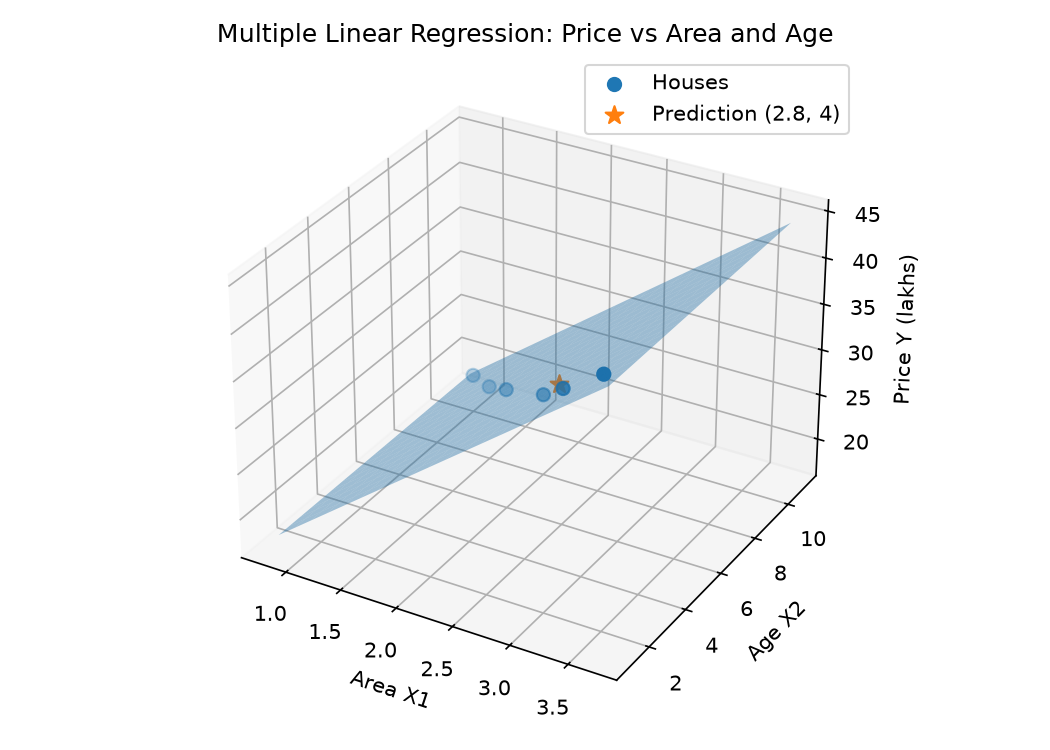
\includegraphics[width=0.78\textwidth]{exp6_plane.png}\par
\small Fig. 1: Houses, fitted plane and predicted house (star).\par
\end{center}
\vspace{4pt}

\expheading{RESULT}
\vspace{4pt}
{\fontsize{12}{15}\selectfont
The above program was implemented and executed successfully using Python, and the corresponding output was obtained and verified. The results of the \textbf{multiple linear regression} were analyzed and found to be satisfactory, thereby achieving the desired objective of the experiment.\par
}

\vspace{12pt}

\noindent\textbf{Faculty Signature:} \underline{\hspace{3.6cm}} \hfill \textbf{Date:} \underline{\hspace{2.8cm}}\par

\end{document}
